\documentclass{thesisclass}
% Based on thesisclass.cls of Timo Rohrberg, 2009
% ----------------------------------------------------------------
% Thesis - Main document
% ----------------------------------------------------------------


%% -------------------------------
%% |  Information for PDF file   |
%% -------------------------------
\hypersetup{
 pdfauthor={?},
 pdftitle={?},
 pdfsubject={?},
 pdfkeywords={?}
}


%% ---------------------------------
%% | Information about the thesis  |
%% ---------------------------------

\newcommand{\myname}{Leon Jungemeyer}
\newcommand{\mytitle}{Rotationally invariant neural networks for homogeneous catalysis}
\newcommand{\myinstitute}{Institute of Theoretical Informatics}

\newcommand{\reviewerone}{?}
\newcommand{\reviewertwo}{?}
\newcommand{\advisor}{Chen Zhou}
\newcommand{\advisortwo}{Pascal Friederich}

\newcommand{\timestart}{24th April 2020}
\newcommand{\timeend}{25th April 2020}


%% ---------------------------------
%% | Commands                      |
%% ---------------------------------

\newtheorem{definition}{Definition} \numberwithin{definition}{chapter}
\newtheorem{theorem}[definition]{Theorem}
\newtheorem{lemma}[definition]{Lemma}
\newtheorem{corollary}[definition]{Corollary}
\newtheorem{conjecture}[definition]{Conjecture}


%% --------------------------------
%% | Settings for word separation |
%% --------------------------------
% Help for separation:
% In german package the following hints are additionally available:
% "- = Additional separation
% "| = Suppress ligation and possible separation (e.g. Schaf"|fell)
% "~ = Hyphenation without separation (e.g. bergauf und "~ab)
% "= = Hyphenation with separation before and after
% "" = Separation without a hyphenation (e.g. und/""oder)

% Describe separation hints here:
\hyphenation{
% Pro-to-koll-in-stan-zen
% Ma-na-ge-ment  Netz-werk-ele-men-ten
% Netz-werk Netz-werk-re-ser-vie-rung
% Netz-werk-adap-ter Fein-ju-stier-ung
% Da-ten-strom-spe-zi-fi-ka-tion Pa-ket-rumpf
% Kon-troll-in-stanz
}


%% ------------------------
%% |    Including files   |
%% ------------------------
% Only files listed here will be included!
% Userful command for partially translating the document (for bug-fixing e.g.)
\includeonly{
titlepage,
introduction,
preliminaries,
content,
conclusion,
appendix
}


%%%%%%%%%%%%%%%%%%%%%%%%%%%%%%%%%
%% Here, main documents begins %%
%%%%%%%%%%%%%%%%%%%%%%%%%%%%%%%%%
\begin{document}

% Remove the following line for German text
\selectlanguage{english}

\frontmatter
\pagenumbering{roman}
%% titlepage.tex
%%

% coordinates for the bg shape on the titlepage
\newcommand{\diameter}{7}
\newcommand{\xone}{-15}
\newcommand{\xtwo}{160}
\newcommand{\yone}{15}
\newcommand{\ytwo}{-253}

\begin{titlepage}
% bg shape
\begin{tikzpicture}[overlay]
\draw[color=gray]  
 		 (\xone mm, \yone mm)
  -- (\xtwo mm, \yone mm)
 arc (90:0:\diameter mm) 
  -- (\xtwo mm + \diameter mm , \ytwo mm) 
	-- (\xone mm + \diameter mm , \ytwo mm)
 arc (270:180:\diameter mm)
	-- (\xone mm, \yone mm);
\end{tikzpicture}
	\begin{textblock}{10}[0,0](4,2.5)
		
\includegraphics[width=.3\textwidth]{logos/KITLogo.pdf}
	\end{textblock}
        \begin{textblock}{10}[0,0](14.5,2.45)
		
\includegraphics[width=.15\textwidth]{logos/algoLogo.pdf}
	\end{textblock}
	\changefont{phv}{m}{n}	% helvetica	
	\vspace*{3.75cm}
	\begin{center}
		\Huge{\mytitle}
		\vspace*{2.25cm}\\
		\Large{
			\iflanguage{english}{Bachelor Thesis of}			
												  {Diplomarbeit\\von}
		}\\
		\vspace*{1cm}
		\huge{\myname}\\
		\vspace*{1cm}
		\Large{
			\iflanguage{english}{At the Department of Informatics}			
													{An der Fakult\"at f\"ur Informatik}
			\\
			\myinstitute
		}
	\end{center}
	\vspace*{1cm}
\Large{
\begin{center}
\begin{tabular}[ht]{l c l}
  % Gutachter sind die Professoren, die die Arbeit bewerten. 
  \iflanguage{english}{Reviewers}{Erstgutachter}: & \hfill & \reviewerone\\
  \iflanguage{english}{}{Zweitgutachter:} & \hfill & \reviewertwo\\
  \iflanguage{english}{Advisors}{Betreuende Mitarbeiter}: & \hfill & \advisor\\
  \iflanguage{english}{}{} & \hfill & \advisortwo\\
  % Der zweite betreuende Mitarbeiter kann weggelassen werden. 
\end{tabular}
\end{center}
}


\vspace{2cm}
\begin{center}
\large{\iflanguage{english}{Time Period}{Bearbeitungszeit}: \ \timestart{} \ -- \ \timeend}
\end{center}


\begin{textblock}{10}[0,0](4,16.8)
\tiny{ 
	\iflanguage{english}
		{KIT -- The Research University in the Helmholtz Association}
		{KIT -- Die Forschungsuniversit\"at in der Helmholtz-Gemeinschaft}
}
\end{textblock}

\begin{textblock}{10}[0,0](14,16.75)
\large{
	\textbf{www.kit.edu} 
}
\end{textblock}

\end{titlepage}

\blankpage

%% -------------------------------
%% |   Statement of Authorship   |
%% -------------------------------

\thispagestyle{plain}

\vspace*{\fill}

\centerline{\textbf{Statement of Authorship}}

\vspace{0.25cm}

Ich versichere wahrheitsgemäß, die Arbeit selbstständig verfasst, alle benutzten Hilfsmittel vollständig und genau angegeben und alles kenntlich gemacht zu haben, was aus Arbeiten anderer unverändert oder mit Abänderungen entnommen wurde sowie die Satzung des KIT zur Sicherung guter wissenschaftlicher Praxis in der jeweils gültigen Fassung beachtet zu haben.

\vspace{2.5cm}

\hspace{0.25cm} Karlsruhe, \today

\vspace{2cm}

\blankpage

%% -------------------
%% |   Abstract      |
%% -------------------

\thispagestyle{plain}

\begin{addmargin}{0.5cm}

\centerline{\textbf{Abstract}}

This thesis finds rotationally invariant features of catalysts using their 3D representation. Using a catalysts unique shape, features are extracted so that spacial orientation of the molecule is of no significance. The generated features are then used to train a neural network that predicts properties of the molecule.

\vskip 2cm

\centerline{\textbf{Deutsche Zusammenfassung}}

Kurze Inhaltsangabe auf deutsch.

\end{addmargin}

\blankpage

%% -------------------
%% |   Directories   |
%% -------------------

\tableofcontents
\blankpage

%% -----------------
%% |   Main part   |
%% -----------------

\mainmatter
\pagenumbering{arabic}
%% LaTeX2e class for student theses
%% sections/content.tex
%% 
%% Karlsruhe Institute of Technology
%% Institute for Program Structures and Data Organization
%% Chair for Software Design and Quality (SDQ)
%%
%% Dr.-Ing. Erik Burger
%% burger@kit.edu
%%
%% Version 1.3.5, 2020-06-26

\chapter{Introduction}
\label{ch:Introduction}

%% -------------------
%% | Example content |
%% -------------------

Catalysts in combination with chemical reactions are used to speed up a reaction by lowering its activation energy. 
Catalysts have an activation energy themselves that needs to be overcome in order to start the reaction, the so called reaction barrier.

The catalyst molecules observed in this thesis are part of Vaska's complex, a chemical compound consisting of a variety of different catalysts all with an iridium atom at their center.
The activation barrier depends on the structure of the catalyst, and varies greatly between different molecules.
Seemingly small changes in the catalysts shape can have a large influence on the catalysts activation barrier [Figure~\ref{fig:struct-diff}].
A rule to guess the activation barrier from the molecules structure cannot easily be found.  
Knowing how to change catalyst molecules in order to lower their activation barrier is a difficult challenge, even to humans.
While the activation barrier can be computed, this process is highly complex and takes a lot of computing power.
This means computing the activation barrier for large datasets of catalysts is currently not feasible.
\\
In this Bachelor's thesis, different approaches to use machine learning to compute the activation barrier of catalyst molecules are explored.
Multiple methods of encoding catalyst molecules into machine-understandable formats are proposed.
Using artificial neural networks, the activation barrier is predicted from the catalysts shape.

After being able to predict the activation barrier with high accuracy, different techniques to explain the 
outputs of the neural network are used.
This helps to better understand booth the network that is usually regarded as a black box, and the feature space.
The explainers used here are simple gradient based methods, and SHAP explainers \cite{NIPS2017_7062}.
This allows for intuition on which parts of the catalyst molecule contribute to the prediction of the activation barrier.
This intuition may be helpful in further chemical analysis of the metal catalyst and can help to give the 
chemist an idea on how an element needs to be changed in oder to lower it's activation barrier.
\\

\begin{figure}
  \centering
  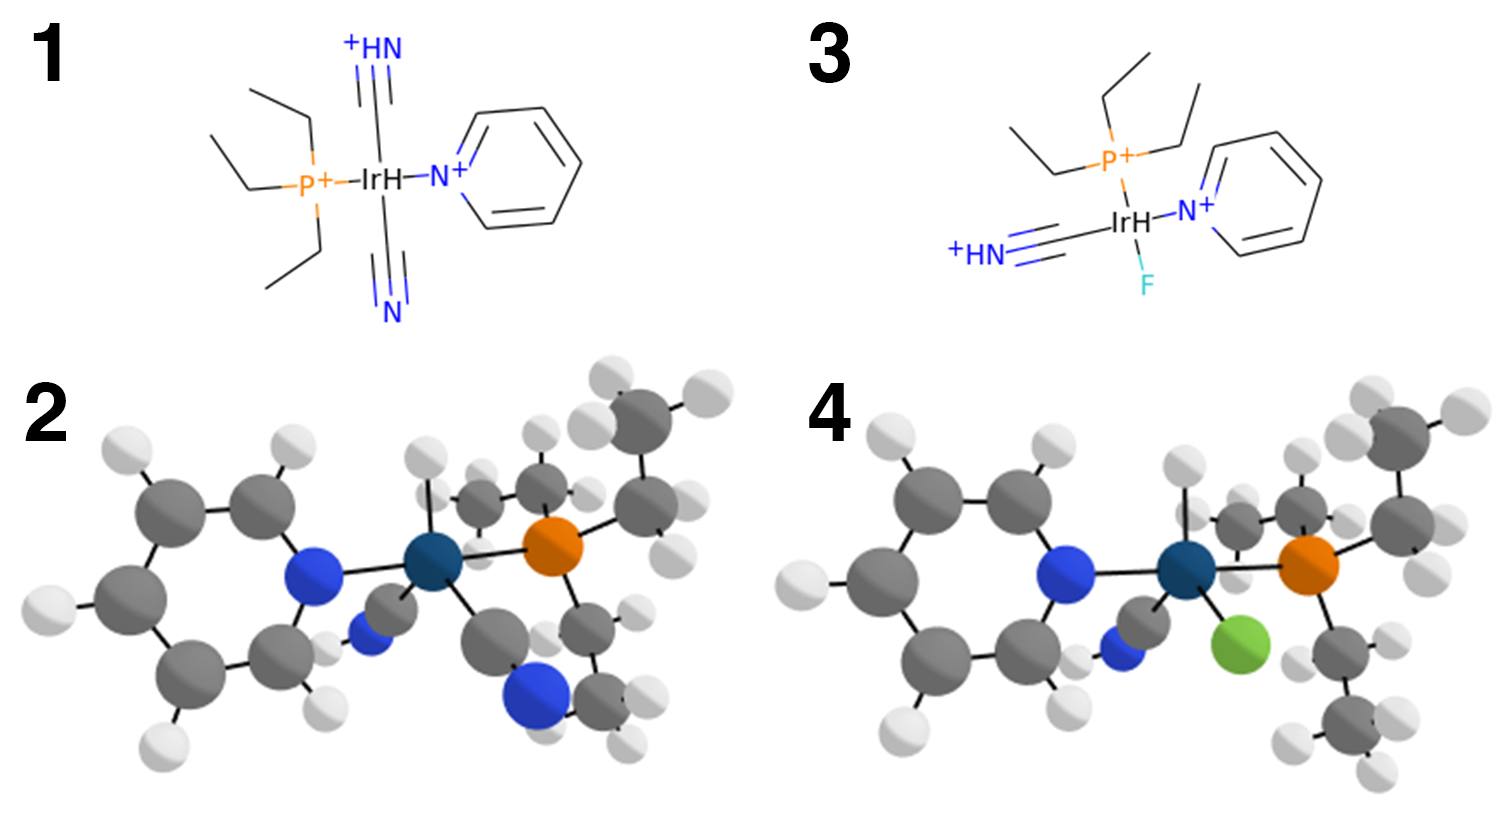
\includegraphics[width=0.8\textwidth]{figures/introduction/elems_intro.png}
  \caption[Example of catalyst molecules]{Two elements with seemingly very similar chemical structures. The chemical structure 1 and it's corresponding 3D structure 2 have an activation barrier of $3.6 kcal/mol$.
  Molecule 3 and it's corresponding 3D structure 4 have an activation barrier of $18.0 kcal/mol$.
  The only difference in the 3D structure of the 2 is the fluorine arm is being replaced by a nitrogen arm.
  The difference is significant considering the distribution of the activation barriers in \ref{fig:barriers}.  }
  \label{fig:struct-diff}
\end{figure}


The metal catalysts in question are constructed by combining different ligands around a central Iridium atom.
As illustrated in Figure~\ref{fig:chemspace}, the central atom has multiple locations that allow different types of ligands to be attached to.  
It enables a quick generation of thousands of different catalyst molecules.
By adding more ligands, the dataset can be increased in size with little effort.
For all catalysts in the dataset the activation barrier, along with other properties, is then computed.
The structure, both chemical and spacial, and the activation barrier is know for every example in the dataset. 
\\
As with many machine learning tasks, feature selection is one of the big challenges in this project.
While there are many universal techniques to extract features from chemical structures, they all have their drawbacks.

In previous works, multiple different techniques are proposed to extract features from a catalyst molecule \cite{friederich_dos}.
These techniques are based on the chemical structure of a molecule, but do not take into account its 3D spacial structure.
This withholds a lot of information to the neural network that might help it to predict more accurately the activation barrier.
The feature extracting methods developed in this bachelor thesis will rely heavily on the 3D structure of the molecule.
The hypothesis is that the 3D structure is playing an important role in the activation barrier, and encoding the 3D structure will enhance regression accuracy.
Additionally encoding 3D structure will allow to learn about the space surrounding the central 
iridium atom to understand the importance of location of the atoms in our molecule.

In order to use feature explainers on the neural network, a reverse mapping from feature space and chemical space needs to be possible.
There currently is no widespread way to encode catalyst molecules that also allows for 
reconstruction of the 3D space and by that an intuition on how the molecule needs to be changed in order ot lower the activation barrier.
Since most chemical feature generators do not specifically focus on catalyst molecules,
but rather provide features for a wide variety of molecules, they generally tend to generate a fully rotational invariant output.
This full rotational invariance means that information about the location of single atoms is often lost or only implicitly encoded in the features.
Therefore a reconstruction of the molecule only from the features is not possible.
The descriptors proposed here allow make use of a catalysts special structure.
This enables a partial reconstruction of the 3D shape of the molecule.
In the future this approach could be used to also encode other properties of the molecule.
\\

The seemingly arbitrary distribution of activation barriers among catalyst molecules  was reason to use neural networks for prediction from the generated features.
Neural networks have become the go-to method for high dimensional regression and classification for their ability to adapt well to complex data.
\\
A limitation of neural networks however is their fixed-size input space.
Therefor a representation of the catalyst needs to be found that encodes molecules into a fixed-size set of features.
These features will then be fed into a neural network for training. 
\\
3D structural encoding comes with its own set of challenges. 
Since a molecules activation barrier does not change depending on its rotation or location in space, 
information about rotation and translation should ideally not be part of the molecules features.
\\
In the case of the metal catalysts, achieving translational invariance is trivial.
Since every catalyst is constructed around exactly one metal atom, the molecule can be centered around this metal atom.

For rotational invariance the problem is more complex.
Every catalyst has a reaction pocket attached to its cental atom.
This reaction pocket has a fixed position.
With the vector from the center of the iridium atom to the center of the reaction pocket, two more degrees of freedom can be removed.
There is no natural way to get rid of the last degree of freedom, rotations around this vector.
%TODO: Figure
Here, 2 different approaches to this last degree of freedom are explored.
The first is using a descriptor that is invariant under rotations around the last degree of freedom.
This removes the need for further normalizations, since all features generated by this descriptor will be invariant.

The second is using data augmentation to teach the neural network about all possible rotations.
This means the molecule is rotated along the last remaining axis of freedom, and and multiple examples of the same molecule at different rotations are used as training examples for the neural network.
This ideally allows the network to abstract away the rotation of a molecule.

After completion of training the networks are able to predict a catalysts activation barrier from its 3D structure.
The main motivation behind encoding the 3D structure is based on the ability to analyse the networks after training.
By analyzing on which features the network is basing its prediction, and translating these features back into 
3D space, we can get an intuition on which parts of the molecule influence its activation barrier.

Additional information about the influence of different species can be gained 
from separately encoding different atom species into their own set of features.

\section{Dataset}

The dataset used for training and testing contains a total of 1947 samples.
Each sample describes the 3D structure of one catalyst molecule, 
containing the position for every atom in that molecule.
Additional information about the molecule was precomputed among the reaction barrier focused on in this work [Figure~\ref{fig:barriers}].
The number of atoms forming one molecule varies between catalysts.
What's consistent is the central iridium atom and the reaction pocket, a single hydrogen atom, attached to the center.
The global position and rotation of the molecule within the dataset is seemingly arbitrary.
Global rotation and location of the element does not influence its activation barrier.
However the local position of atoms in the molecule plays and important role in the activation barrier.

\begin{figure}
  \centering
  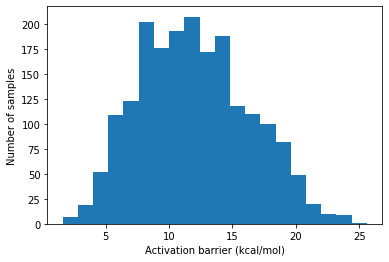
\includegraphics[width=7cm]{figures/introduction/barrier.png}
  \caption[Distribution of activation barriers]{Distribution of the elements activation barrier. The elements have a mean of $11.970 kcal/mol$ and a standart deviation of $4.33 kcal/mol$.}
  \label{fig:barriers}
\end{figure}

The dataset was constructed from a set of ligands.
These ligands are placed around the iridium core in a specific order.
There is a total of 3 ligand groups, with every group being able to attach in a different way to the metal center.
By combining different ligands from these groups, catalysts are created [Figure~\ref{fig:chemspace}].
These chemical structures are known as Vaska's complex.

Due to this combinatorial approach the dataset could later be increased with relatively low effort.
The biggest hurdle to increasing the dataset size is computing the activation barrier.
This computation is highly complex and therefore not feasible for large datasets.
However, generating a larger dataset without computing the activation barrier could still be helpful when using transfer learning approaches to fine tune the network.
This idea is further discussed in [Chapter~\ref{ch:Conclusion}].

\begin{figure}
  \centering
  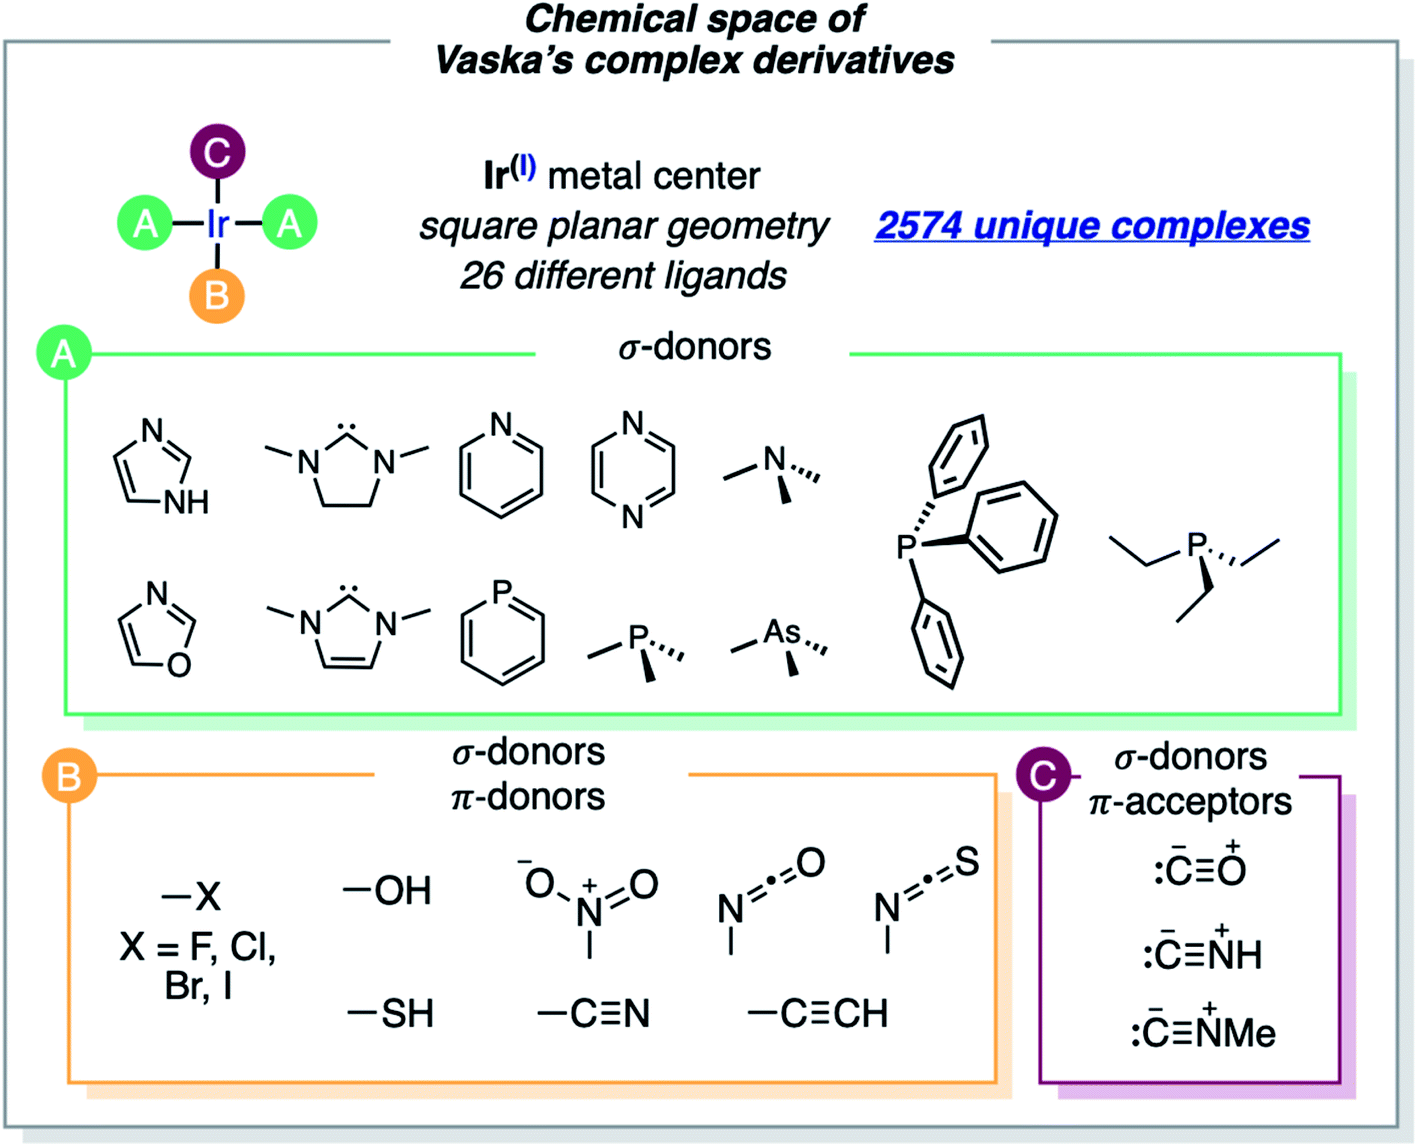
\includegraphics[width=10cm]{figures/introduction/chem-space.png}
  \caption[Vaska's space]{Ligands defining the chemical space associated with Vaska's complex. Reprinted from \cite{friederich_dos}.}
  \label{fig:chemspace}
\end{figure}


\section{Previous research}

In previous approaches different machine learning methods were used to predict the activation barrier of the elements in this dataset.
The features extracted from the elements focused on their atomic properties.
However, the features extracted from the molecule did not take into account the spacial structure of the element.
The elements were instead encoded by creating a graph from the chemical structure.
The elements are then grouped by their distance from the metal center.
For each group of elements, features were computed as sum of pairwise products/differences of their atomic properties(such as electronegativity, atomic number, identity, topology and size) \cite{friederich_dos}.
Note that these features do not contain any information about the 3D location of the atoms.

Using these autocorrelation features, a neural network and other forms of regression were used to predict the activation barrier.
Gaussian processes were able to predict the activation barrier within an error of $<1 kcal/mol$ for a train split of $80\%$.

In a unpublished approach, the autocorrelation features were replaced by a graph structure of the molecule.
On this graph structure, a graph convolutional neural network was trained.
When training on a large fraction of the dataset this network reached accuracies 
beyond what could be achieved using autocorrelation features, reaching accuracies of $<0.5 kcal/mol$ for a training fraction of 90\%.

All of these methods used features independent of the 3D structure of the element.
Other than the obvious disadvantage of withholding information from the element, another disadvantage is the lack of interpretability of results.
While these features succeed at predicting reaction barriers, gaining 
information about what part of the molecule is contributing to the prediction is limited or not possible.

The feature extractors introduced in this thesis aim to solve this problem by extracting features that allow for a
partial reconstruction of the chemical space.
This helps to better understand the origin of a prediction, and might be helpful to better understand 
the underlying elements in a chemical sense.

Feature extraction is a common problem for machine learning methods in chemical spaces.
Multiple approaches have been proposed for general molecule encoding, 
ranging from encoding properties of molecules, such as the Coulomb Matrix encoder encoding electrostatic interaction of atoms \cite{PhysRevLett.108.058301}
to encoding 3D structures of atomic environments \cite{Bart_k_2013}.

3D structural encoders usually create a fully rotational invariant features.
In the case of SOAP proposed by \citeauthor{Bart_k_2013}, this is achieved by encoding information about the interaction of 
different species rather than encoding the 3D space itself.
Fully invariant 3D descriptors have the advantage of being universally applicable for any kind of molecule, since they have no requirements to the element being encoded.
The disadvantages are that, once the features are generated, a transformation back to 3D space is usually not possible.
In many applications, this is not a problem since the generated features are used only for prediction of an elements properties.
In the applications here the features however should later allow to interpret the 3D space surrounding the molecule and ideally give an idea on how the molecule can be changed to alter its properties.

The idea of using a catalysts special structure for this task, and therefore removing some axes of freedom from the feature space, seems to be an unexplored approach.

Since the structure of the catalyst still leaves 1 degree of freedom, the prediction needs to be partly rotationally invariant.
This is a common problem for neural networks even outside of chemistry.
Generally the approaches to solving these problems can be divided into 2 different groups.

The first being feature engineering to generate features from the data that are fully invariant of rotation.
In point clouds approaches include representing the data as angles and distances rather than the points itself \cite{weiler20183d, 8886052}.
Since these features do not change depending on the rotation and translation of the points, the network does not need to 
abstract away the rotational information of the data.
While this method guarantees full rotational invariance, it requires extensive feature engineering.
Additionally, it may increase complexity of the features and in many cases 
goes hand in hand with the loss of some information from the original dataset. 
Restoring the original data is therefore often impossible.
%The EFD feature generator proposed here implements a fully rotationally invariant description by using 
%descriptor that can be normalized for rotation.

A second approach to rotational invariance is data augmentation.
In image recognition data augmentation has already become the go-to method.
Data augmentation removes the need for extensive feature engineering.
Instead, the training data is augmented along all axes of freedom.
In the case of image recognition, this means rotating, scaling, and in some cases deforming the input images.
By that, the dataset will be filled with more examples for every data point, and ideally the model is able to 
abstract away these features. %TODO: Citation needed
In the case of catalyst molecules, each element will be rotated around the remaining axis of freedom.
The different angles will then be fed into to the network for training.
%The SNAP feature generator proposed here produces a partially rotationally invariant output that needs to be augmented along one axis.
%All the augmentation steps are then fed to the networks in order to teach the network to abstract away the different rotations of the catalyst.

\section{Objectives}

As with many machine learning tasks, using the raw data as input to machine learning models is not feasible.
Features are therefore generated from the raw data that can be used to learn from.
The typical workflow for machine learning in chemical fields reflects this approach [\ref{fig:feature-process}].

This work can be grouped into 3 main objectives. 
The first is to find a feature extractor that generates features from a catalyst molecule that ideally rotationally invariant.
The second objective is to train a neural network on these features that predicts the activation barrier.
The goal was to achieve accuracy similar or higher to what \citeauthor{friederich_dos} achieved in \cite{friederich_dos}.
In a final step, using explainers to explain the origins of the networks prediction, an intuition on how a catalyst has 
to be adapted in order to change it's activation barrier is given.


\begin{figure}
  \centering
  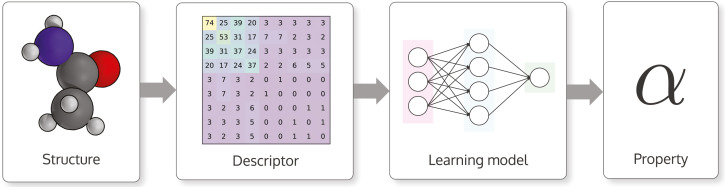
\includegraphics[width=12cm]{figures/introduction/chem-descriptor.jpg}
  \caption[Machine learning in chemistry]{Visualization of feature generation and prediction from the generated features. 
  A fixed size descriptor is generated from the structure. Using machine learning techniques, 
  predictions are made from these features.
  The feature generators proposed here should allow a partial inversion of this process to allow for interpretability of the results.
  Reprinted from \cite{dscribe}.}
  \label{fig:feature-process}
\end{figure}


\subsection{Feature generation}

The features should allow a regressor to make predictions from the 3D shape of the molecules.

Therefor features have to be of fixed length for all elements in the dataset.
The amount of atoms in one element cannot influence the number of features.

Ideally the number of features is as low as possible, helping the model to identify the relevant features better.
The number of features cannot be too small as it should still contain all relevant information.
For interpretability of the results, the features should allow for a partial or full reconstruction of the element they are encoding.
This means, given the features, it should be possible to approximate the general shape of the molecule.

To allow for computational exploration of the encoded space, the features should be continuos.
Small changes in the density space should result in small changes in the 
feature space. 
This means hashing from chemical space to feature space is not viable.

The global location and rotation of the element should not influence the features or have only limited influence on the features.

Two different approaches to feature generation are prosed.
The first is a fully rotationally invariant output using a rotationally invariant contour description.
While the output of this descriptor is fully invariant, it suffers from sampling issues due to the nature of it's encoding.

The second approach to feature generation was using a combination of basis functions to fully describe a local environment around a central atom.
Using a set of coefficients, the density space surrounding the central atom can be approximated.

\subsection{Regression}

The second step is to predict the activation barrier from these features using an artificial neural network.
A reference for prediction accuracy was set by \cite{friederich_dos}.
The networks proposed here achieve higher accuracy's than the best regression methods proposed in \cite{friederich_dos}.

The regression methods performed on features created with method \ref{ch:SNAP} achieve accuracies higher than regression methods on graph convolutions,
the highest accuracy regressors on this dataset to date.

\subsection{Explaining the feature space}
Since the features should be able to allow a inversion back to the 3D space, it's possible to approximate which areas in 3D space are responsible for the prediction.
Using neural networks explainers, in  a last step the regions in 3D space that influence the regression will be analyzed.
This gives an idea on how different atoms in the dataset influence the prediction.
Looking at the gradient of the input with respect to the activation barrier, an intuition on how the catalyst molecule needs to be 
adapted in order to decrease the activation barrier can be given.

Due to the low resolution of the encoder, the information that can be gained is limited.
%% preliminaries.tex
%%

%% ==============
\chapter{Preliminaries}
\label{ch:preliminaries}
%% ==============

This chapter should provide the foundations of the thesis.
%% LaTeX2e class for student theses
%% sections/content.tex
%% 
%% Karlsruhe Institute of Technology
%% Institute for Program Structures and Data Organization
%% Chair for Software Design and Quality (SDQ)
%%
%% Dr.-Ing. Erik Burger
%% burger@kit.edu
%%
%% Version 1.3.5, 2020-06-26

\chapter{Feature generation}
\label{ch:features}
%% ==============
Artificial neural networks(ANNs) and other machine learning techniques have strict requirements to their input data.
For ANNs specifically, the input needs to be of fixed size and ideally as low dimensional as possible.
To achieve that, a fixed number of features are extracted from the molecules.
In order to learn, all the data required to predict molecular properties, in this case the activation barrier, should be encoded in the features.
These features can then be used to train a neural network.

Simple encoders extract well know features of molecules such as their mean electro negativity or atomic numbers \cite{LO20181538}.
Approaches by state-of-the-art chemical encoders include using graph convolutions to parse the chemical structure into fixed size features \cite{GNN_ENCODER}.
Others try to encode interaction of different atoms or species of atoms into their features \cite{PhysRevLett.108.058301}.
The feature generators relevant to this project are spacial encoders.

Spacial encoders in chemistry generally focus on describing the interaction of chemical elements within a certain radius, rather 
than the space itself \cite{Bart_k_2013}.
Since global rotation and translation of an element generally does not influence it's chemical properties,
encoders try to produce rotationally invariant representations.
This usually limits the possibilities of reconstructing the input data.
A 3D representation can therefore not easily be computed from the generated features.

The feature generators proposed here have the ability to partly reconstruct the 3D space they are encoding.
In order to retain partial rotational invariance the special structure of the input data is used.
All catalyst molecules in the dataset have a central metal atom and a reaction pocket composed of a hydrogen atom attached to the metal center.
By the centers of these 2 atoms a unique axis is formed.
This axis is used to align the molecules.

The use of this special structure of catalyst molecules to generate partly invariant features seems to be a novel approach.

After alignment, two different approaches to feature generations are explored.
The first method slices the molecule at certain heights.
The slices are then described using a fully rotationally invariant descriptor.

The second approach is to use a combination of different 3D basis functions to encode the space surrounding the central atom.
Since this description is not fully invariant, data augmentation is used along the remaining axes of freedom.

\section{Alignment of catalyst molecules}

Every catalyst molecule $\mathbb{E}$ in the dataset has a central Iridium atom with position $p_{Ir} \in \mathbb{E}$.
The Iridium atom is set to the center, all other atoms are aligned accordingly.

$$ \forall p_i \in \mathbb{E}: p_i' = p_i - p_{Ir}$$

Now that the element is centered, the next step is rotating it.
Every catalysts has a reaction pocket attached to the central metal atom.
This reaction pocket is defined by a single hydrogen atom attached to the central iridium atom.
The goal is to rotate the entire molecule so that the reaction pocket is aligned with the $z$-Axis.
The axis to be aligned is defined by the vector running from the center to the reaction pocket, so

$$ v = \frac{p_{Pocket}'}{\| p_{Pocket}'\| } $$

The vector $v$ is now rotated so that it aligns with the $z$-Axis.
Since this rotation can be defined no matter the elements initial alignment, it effectively removes rotational invariances.
Let $A$ be a plane through the points $(0,0,0), (0,0,1), v$.
The normal $n$ of $A$ is the axis the molecule will be rotated around.

$$
n =\frac{\begin{pmatrix}
  0 &
  0 &
  1
\end{pmatrix}^T \times v}{ \left\| \begin{pmatrix}
  0 &
  0 &
  1
\end{pmatrix}^T \times v \right\| }
$$
Next, the angle $\alpha$ between $v$ and the $z$-Axis on the plane is computed.

$$ 
\alpha = k \cdot \arctantwo \left( 1,  
\begin{pmatrix} 0 &  0 & 1 \end{pmatrix} \cdot v \right),\space k = \left\{\begin{array}{ll} 1, & n \cdot \left( (0,0,1)^T \times v \right) > 0 \\
  -1, & \text{otherwise}\end{array}\right.
$$

A rotation matrix around the normal $n$ can be defined as:
$$
R(\alpha) = I_3 + C \sin(\alpha) + C^2(1 - \cos(\alpha)), C =
\begin{pmatrix}
  0 & -q_0 & q_1 \\
  q_2 & 0 & -q_0\\
  -q_1 & q_0 & 0
\end{pmatrix}
$$


The rotation $R(\alpha)$ can then be applied to all centered atoms in the element.
The aligned and centered molecule can therefor be described as

$$ 
\mathbb{E}^R = \left\{ R(\alpha) (p_i - p_{Ir}) |  p_i \in \mathbb{E} \right\}
$$

The coordinates $p^R_i \in \mathbb{E}^R$ are now rotationally invariant under 2 axes. 
The only degree of freedom left is rotations around the $z$ axis. 

This normalization is repeated for every element in the dataset.

%Since there's no natural way to align the elements around $z$, different approaches will be used.
%In a first attempt, features are generated using a descriptor that is fully invariant under rotations around $z$.
%The second descriptor is using data augmentation to teach the network about possible rotations of the molecule.





\section{Fourier descriptors for invariant feature generation}

The first attempt at feature generation was using a fully rotational invariant feature descriptor.
The method used is an Elliptic Fourier Descriptor (EFD).
Elliptic fourier descriptors approximate a 2D contour with a set of coefficients.
The higher the order of the descriptor, the better a contour can be approximated.

To be able to describe a 3D object using fourier contour descriptors the object is sliced at different $z$ heights.
For each slice, the contour is described using an EFD.
This generates a fully rotationally invariant description.
Since EFDs allow to approximate a contour with just a few coefficients, the generated features
are also low dimensional.
This feature generator will be referred to as layered elliptic fourier descriptor(LEFD).

\subsection{Slicing}
\begin{figure} [h]
  \centering
  \includegraphics[width=0.5\textwidth]{figures/fourier/slice3D.png} % for .pdf files etc use \includegraphics{test.pdf}
  \caption[Slicing a molecule]{A molecule is sliced by a plane. Every slice is taken at a different $z$ height.}
  \label{fig:slice3D}
\end{figure}

Along the $z$-axis, starting from $z_{start}$ to $z_{end}$, the molecule is sliced in a distance of $z_{height}$.
$z_{start}, z_{end}, z_{height}$ are tuning parameters.
Here, $z_{start}, z_{end}$ are chosen so that all molecules from the dataset fully fit into the boundaries.

A slice is computed by getting the radius of every atom $i$ in the molecule at the slice height $z$ Figure~\ref{fig:slice3D}.

$$ r_i(z) =\left\{\begin{array}{ll} \sqrt{R_i^2 - (z - p_i^R[2])^2} &, | z - p_i^R[2] |  < R_i\\
  0 &, \text{otherwise}\end{array}\right.
$$ %TODO: Der Betrag ist immer > 0 ???

$R_i$ is the Van-der-Waals radius of element $i$, $p_i[2]$ is the $z$ component of the location vector.
The slice is now constructed by drawing a circle with radius $r_i(z)$ around the $x,y$ coordinates for each atom for each slice Figure~\ref{fig:slice}.

\begin{figure} [h]
  \centering
  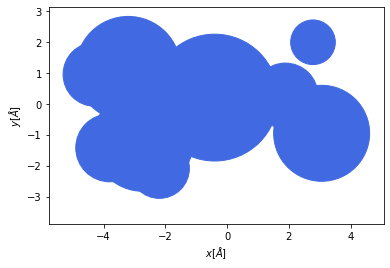
\includegraphics[width=0.5\textwidth]{figures/fourier/slice-iso.png} % for .pdf files etc use \includegraphics{test.pdf}
  \caption[Visualization of a slice with isolates]{A slice with isolates.}
  \label{fig:slice}
\end{figure}

The slice consists of a set of circles.
These circles can be partially or fully intersecting. 

To describe the contour, a fourier contour descriptor is used.
This contour descriptor allows to easily ignore rotation of the contour and generate invariant low-dimensional features from the shape.
However, it can only work on a closed contour, so isolate islands of circles that don't intersect have to be dealt with separately.
For simplicity, islands will be ignored by the contour descriptor.
To identify islands and one continuos subset of circles, for each slice a graph is constructed.
For every atom with radius $>0$ we create a node.
For every atom that intersects with another we create an edge between these two nodes.
Now the \texttt{Largest Connected Component}, so the connected subgraph with the most nodes, is computed.
This gives us the most atoms forming a continuously connected shape in the current slice.
In the next steps we will only use this subset of circles to describe the contour.
%TODO: Not perfect, but good enough?
\paragraph{Finding the contour}

From the set of intersecting circles, the contour needs to be extracted. 
Since the contour points are computed just from radius and position information, and are not rendered onto a 2D pixel grid, standard contour finding algorithms can not be used.
Instead, knowledge about the general shape is used to compute the contour. 

The contour is computed using \autoref{alg:CircleSetContour}.

First, the point "furthest to the right", so with the largest $x$-Value is found. 
Since the point with the highest $x$-Value in any circle is always at angle 0, we set the initial angle $\alpha$ and rotation vector $\vec{p}$ accordingly.
From the circle containing that point, the contour is followed from that point counter-clockwise until the first intersection with another circle is found.
To the list of contour sections, we add the current contour section from angle $0$ to the angle of intersection.

Now, the contour of this circle is followed again until it intersects another. This is repeated until the starting circle is reached again.

Once the starting circle is reached, the last remaining contour part of the starting circle needs to be added to the list of contour sections Figure~\ref{fig:circlesetcontour}.

From the ordered list of contour sections, the contour points can easily be computed.
Since each contour section consist of a radius $r$, location $(x,y)$, and start- and end angle $\alpha_{start}, \alpha_{end}$, the coordinates of the contour points can simply be computed using $x_c = \cos(\alpha_c) \cdot r + x$ and  $y_c = \sin(\alpha_c) \cdot r + y$ 
for $\alpha_c = \alpha_{start} + i \cdot \Delta, \alpha_c \leq \alpha_{end}, i \in \mathbb{N}_0$.

$\Delta$ is a tuning parameter that specifies the resolution of the contour.

This process of going along the outside ignores all "holes" in the shape, so only the outermost contour will be part of the final result. 
This is beneficial since EFDs only allow for the encoding of a single closed contour.

\begin{figure}[!htb]
  \minipage{0.32\textwidth}
    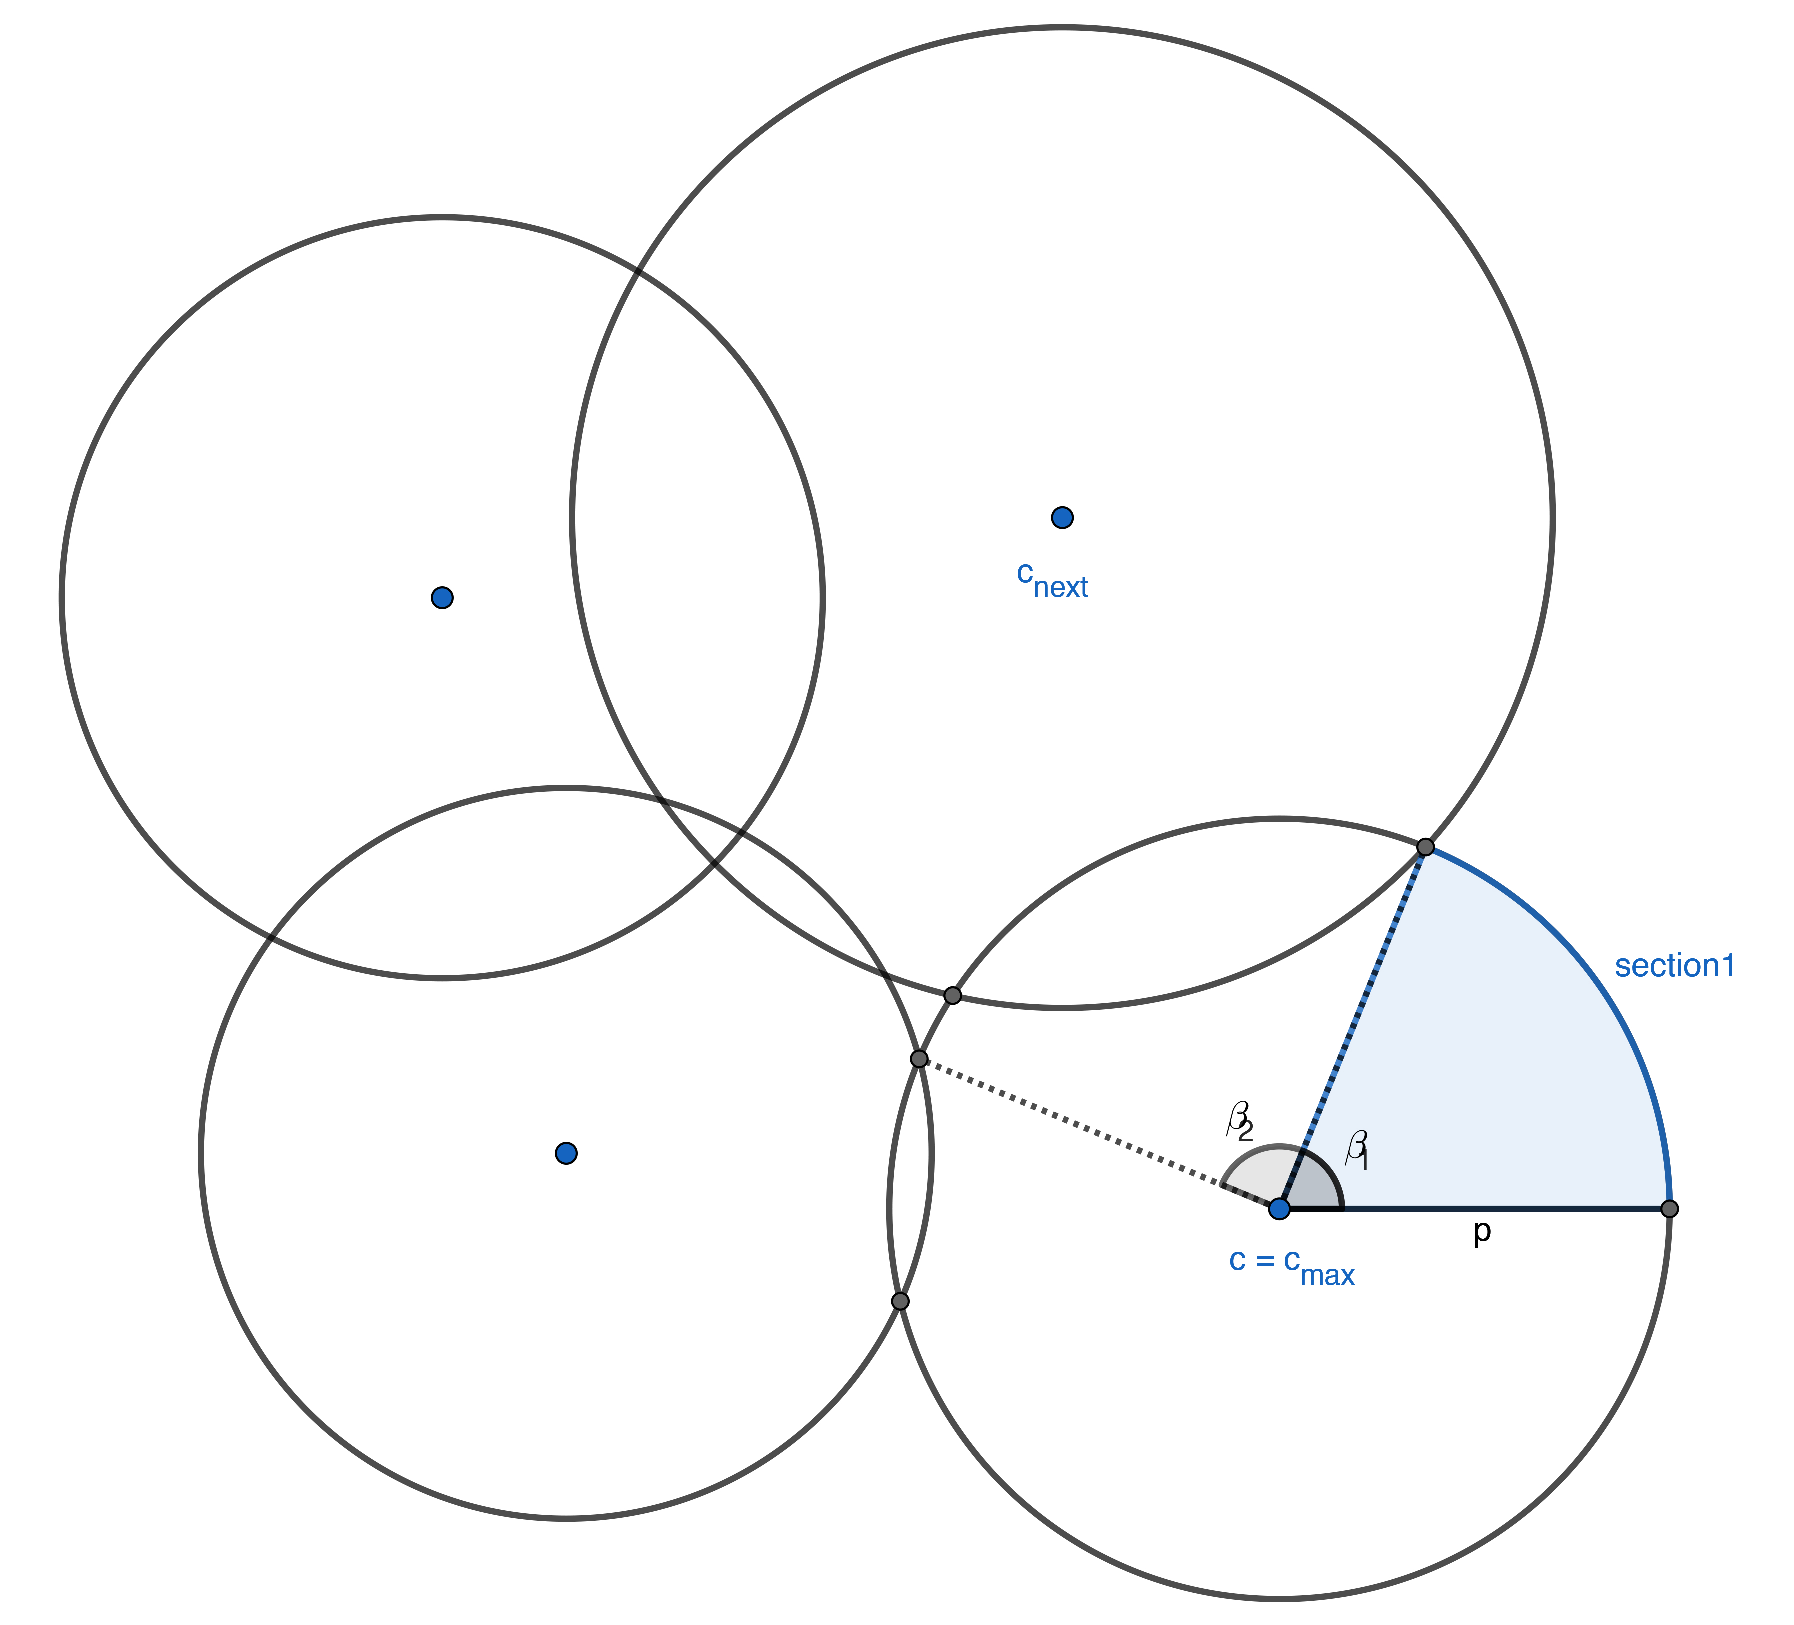
\includegraphics[width=1.0\textwidth]{figures/contour/c1copy.pdf}
    \caption{Finding first contour section}
  \endminipage\hfill
  \minipage{0.32\textwidth}
    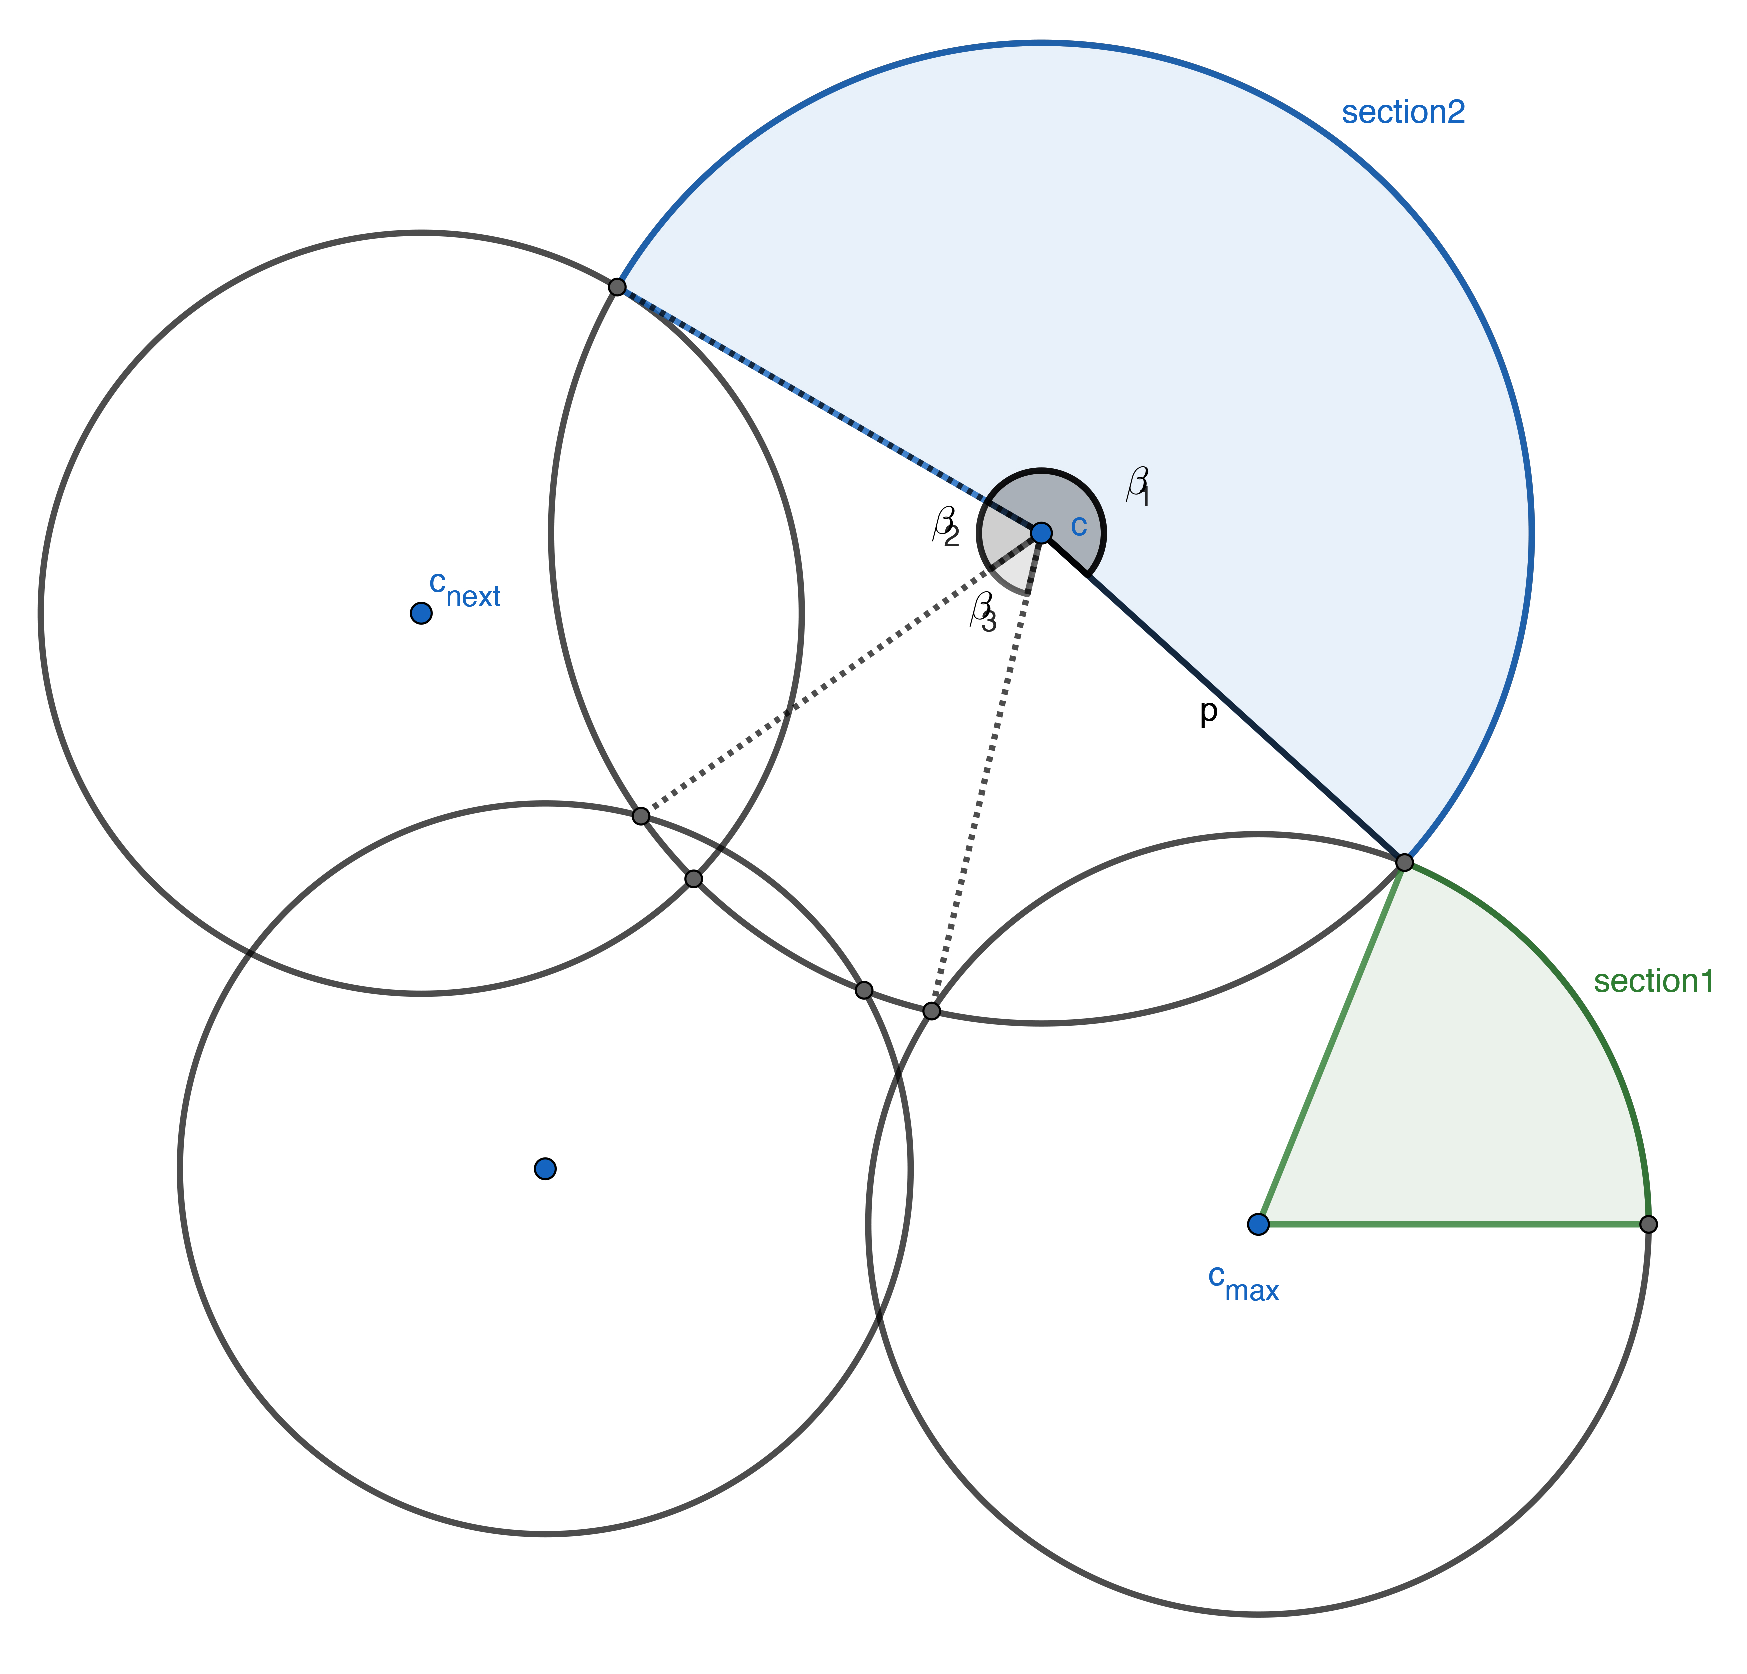
\includegraphics[width=1.0\textwidth]{figures/contour/c2copy.pdf}
    \caption{Finding middle contour section}
  \endminipage\hfill
  \minipage{0.32\textwidth}%
    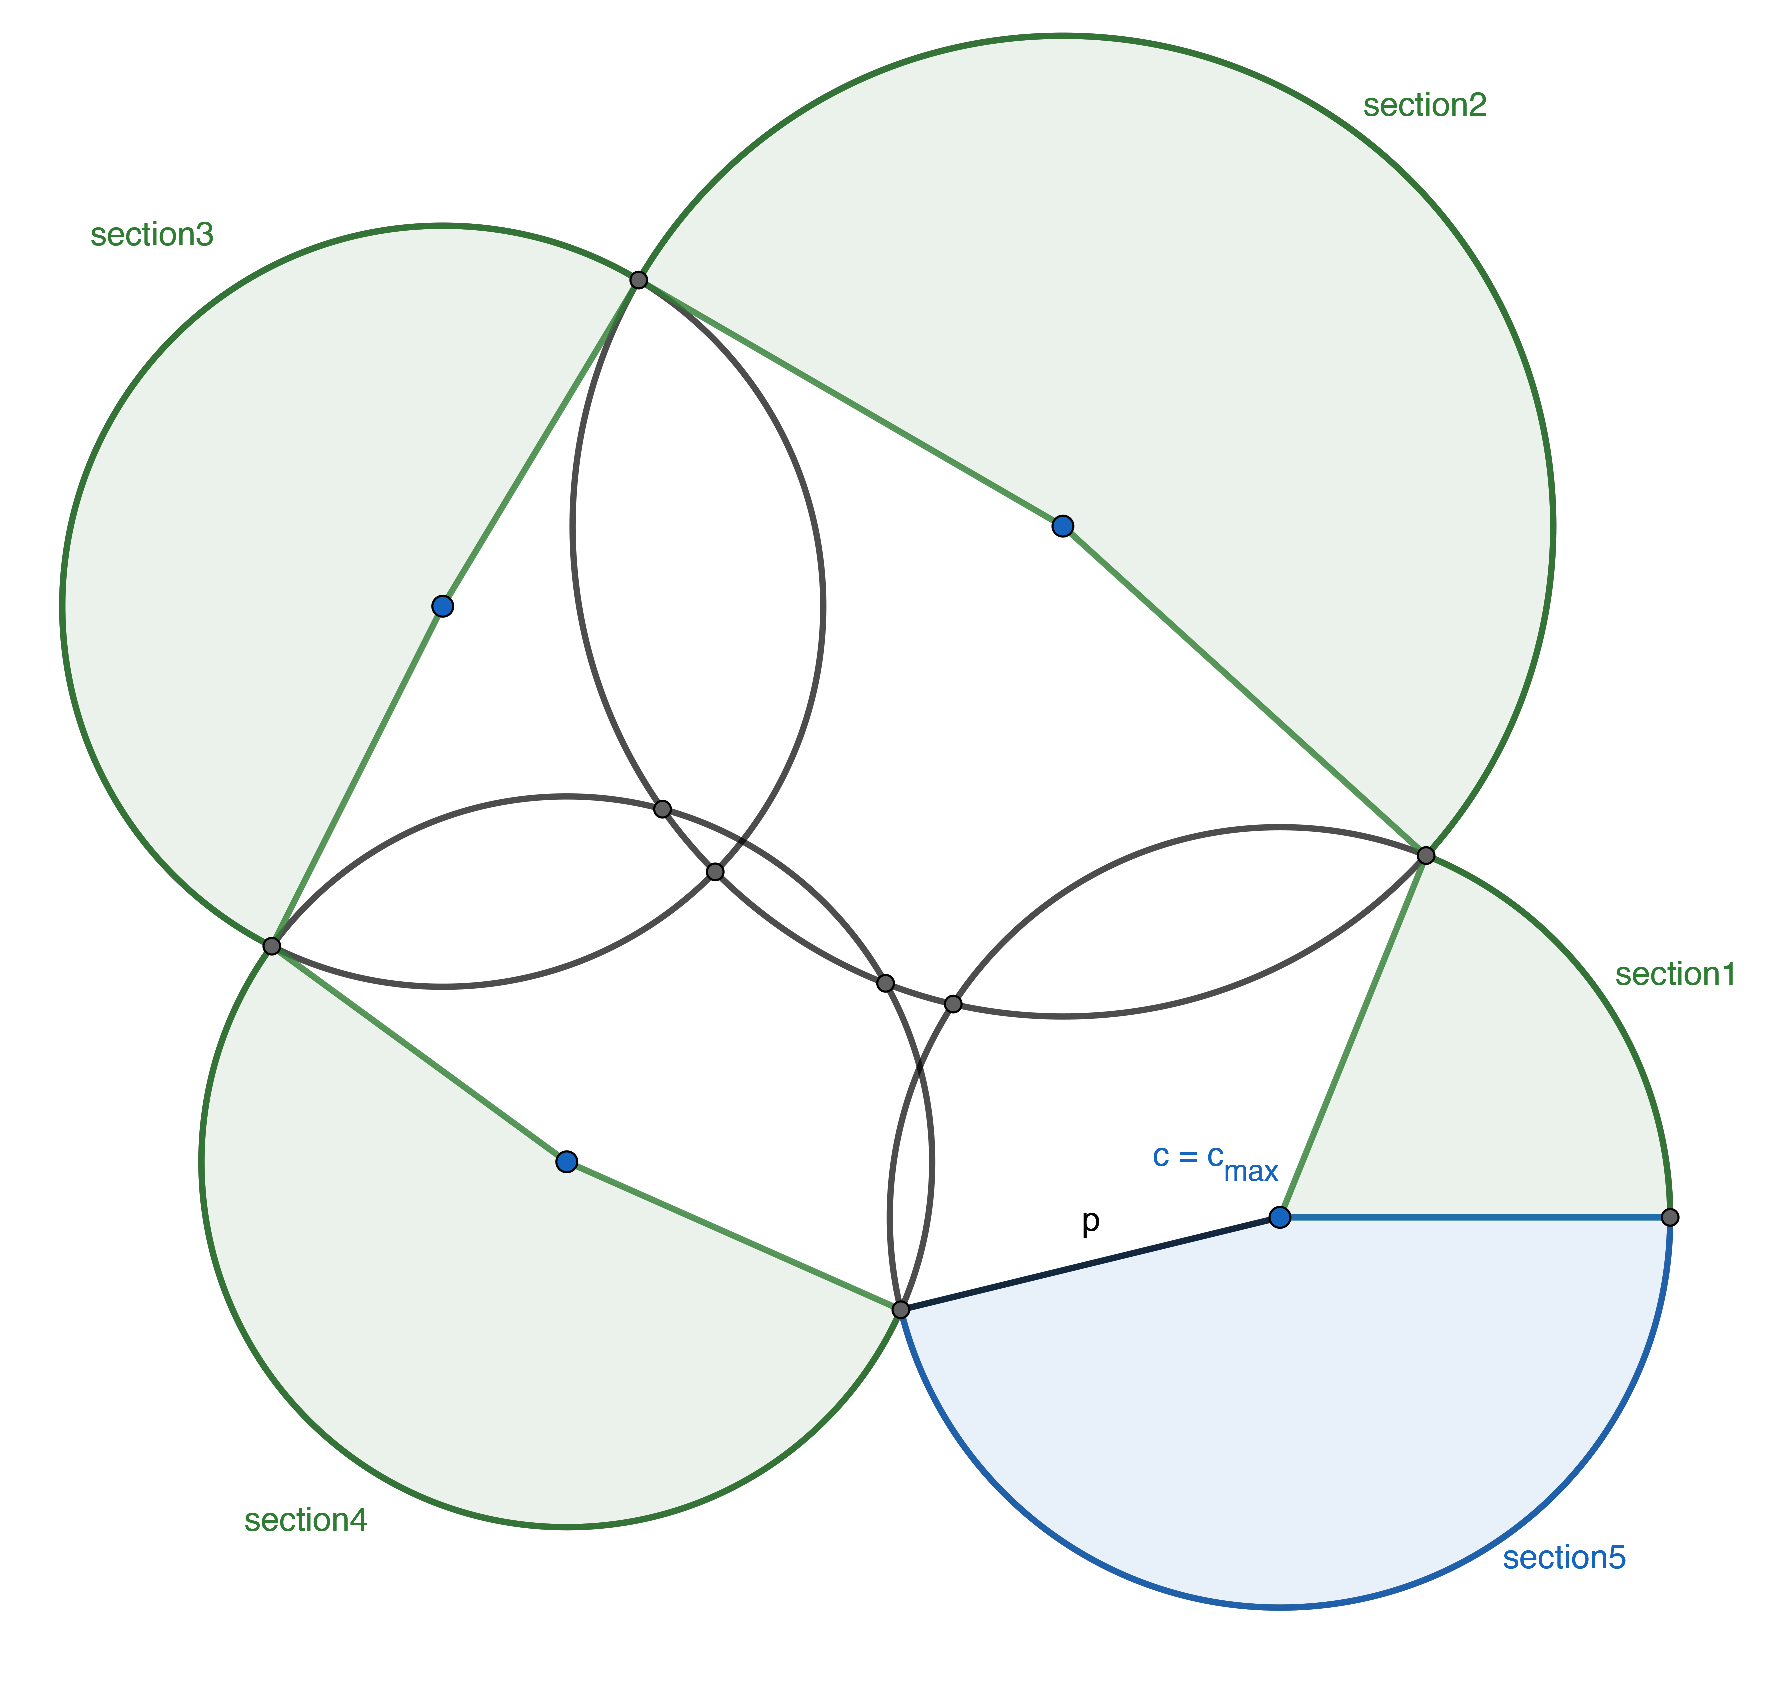
\includegraphics[width=1.0\textwidth]{figures/contour/c3copy.pdf}
    \caption{Finding the last contour section}
  \endminipage
  \caption[Visualization of CircleSetContour algorithm]{Visualization of \autoref{alg:CircleSetContour}}
  \label{fig:circlesetcontour}
\end{figure}


\subsection{Elliptic fourier descriptor}

Now that we have a contour for each slice, we'll use the elliptic fourier descriptor (EFD) to describe that contour.
EFDs allow for a high resolution encoding of a contour in a fixed amount of coefficients.
Additionally, EFD coefficients can easily be made rotationally invariant.

EFDs, as described in \cite{LIN1987535} work by selecting a random starting point $s$ on the contour.
Starting from $s$, we will follow the contour and denote the $x$ and $y$ coordinates as functions $x(l)$, $y(l)$ of the distance $l$ from the starting point.
Distance refers to the length it takes to get from $s$ to the point following the contour.

Since the starting and end point of $x(l), y(l)$ will be equal, making them periodic, we can define a parameter $t=\frac{2\pi l}{n}$. %TODO: Erklären!!!!
The functions can then be described by Fourier expansions as

%TODO: Replace t and put it in directly?
$$
\begin{pmatrix}
  x(l) \\
  y(l) \\
\end{pmatrix}
=
\begin{pmatrix}
  a_0 \\
  d_0 \\
\end{pmatrix}
+
\sum_{k=1}^\infty 
\begin{pmatrix}
  a_k & b_k\\
  c_k & d_k\\
\end{pmatrix}
\cdot
\begin{pmatrix}
  \cos(kt)\\
  \sin(kt)\\
\end{pmatrix}
$$

with

$$
a_0 = \frac{1}{2\pi} \int_{0}^{2 \pi}  x(t) \,dt 
$$
$$
d_0 = \frac{1}{2\pi} \int_{0}^{2 \pi}  y(t) \,dt 
$$

$$
a_k = \frac{1}{\pi} \int_{0}^{2 \pi}  x(t) \cos(kt) \,dt 
$$
$$
b_k = \frac{1}{\pi} \int_{0}^{2 \pi}  x(t) \sin(kt) \,dt 
$$
$$
c_k = \frac{1}{\pi} \int_{0}^{2 \pi}  y(t) \cos(kt) \,dt 
$$
$$
d_k = \frac{1}{\pi} \int_{0}^{2 \pi}  y(t) \sin(kt )\,dt 
$$

The $a_k, b_k, c_k, d_k$ form a basis for the functions $x(l), y(l)$.
By addition of the vector $ \begin{pmatrix} a_0 & b_0 \end{pmatrix}^T $ a center offset can be defined.
Since the contours encoded here should stay rotationally invariant, a two dimensional offset is not feasible.
Instead the offset length $\|  \begin{pmatrix} a_0 & b_0 \end{pmatrix}^T \| $ is added to the feature vector.

So far, the features $a_k, b_k, c_k, d_k$ are depended on the rotation of the contour.
The next step will be to make the features invariant under rotations.
%%%The starting point $s$ does not affect the coefficients as shown by \citeauthor{KUHL1982236}.

The contour can be viewed as a summation of ellipses of different size.
By aligning the first ellipse and rotating all other ellipses accordingly, the final output can be made invariant
of rotation \cite{MEBA}.

$$
\theta = \frac{1}{2}\arctan \left( \frac{2(a_1b_1 + c_1d_1)}{a_1^2 + c_1^2 - b_1^2 - d_1^2} \right)
$$
$$
\psi = \arctan \left( \frac{\cos(\theta) a_1 + \sin(\theta) b_1 }{\cos(\theta) c_1 + \sin(\theta) d_1} \right)
$$

The aligned coefficients $a_k^R, b_k^R, c_k^R, d_k^R$ can then be obtained using

$$
\begin{pmatrix}
  a_k^* & b_k^* \\
  c_k^* & d_k^* \\
\end{pmatrix}
=
\begin{pmatrix}
  \cos(\psi) & -\sin(\psi) \\
  \sin(\psi) & \cos(\psi) \\
\end{pmatrix}
\begin{pmatrix}
  a_k & b_k \\
  c_k & d_k \\
\end{pmatrix}
\begin{pmatrix}
  \cos(k\theta ) & -\sin(k\theta) \\
  \sin(k\theta) & \cos(k\theta) \\
\end{pmatrix}
$$.

The rotation around $\theta $ can be interpreted as normalizing the starting point $v$, 
the rotation around $\psi$ as normalizing the rotation of the contour itself \cite{KUHL1982236}.

The last step is to choose an order up to which the contour is approximated.
At the moment the infinite sum ensures a perfect approximation original contour. 
By limiting the coefficients to an order $k_{max}$ the number of coefficients describing our contour can be limited.
Generally, the higher the order, the better small changes in the contour can be approximated Figure~\ref{fig:slice-layered}.

After normalizing, the values $b_1^* = c_1^* = 1$ will always be equal to 0, since we rotated the first ellipse to be aligned.
We can therefore remove $b_1^*, c_1^*$ from the feature vector.

After calculating the coefficients for every slice, the different slices will be concatenated into a 2D array.
One dimension of the array will correspond to the spacial $z$ direction, so it will be equivalent to the number of layers chosen.
The other dimension will hold the fourier coefficients for each layer.

To keep information about the offset from the center, the length $l = \| \begin{pmatrix} a_0 & b_0 \end{pmatrix} \| $ will be added for each slice.
Since each fourier coefficient consists of 4 values and $b_1^*, c_1^*$ are removed while the center offset $l$ is added, the size of this dimension will be $k_{max} * 4 - 1$.

These features will be used for prediction of a molecules activation barrier in the next step.

\begin{figure}[h]
  \minipage{0.4\textwidth}
    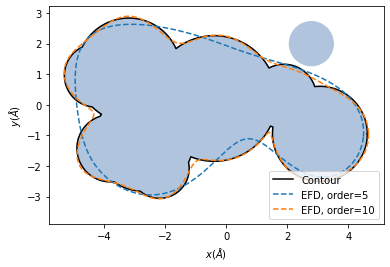
\includegraphics[width=1.0\textwidth]{figures/fourier/contour.png}
  \endminipage\hfill
  \minipage{0.6\textwidth}
    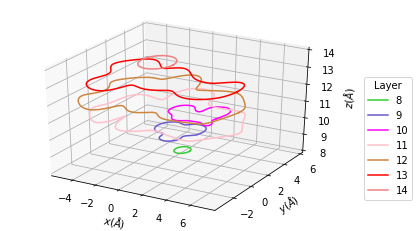
\includegraphics[width=1.0\textwidth]{figures/fourier/fourier-slices.png}
  \endminipage
  \caption[Slices produced by LEFD encoder]{
  On the left a slice is described by fourier descriptors. Higher order descriptors are able to approximate the contour better than lower order descriptors. 
  The isolate is ignored by the contour descriptor. The rotation is kept as part of the fourier description for illustration purposes.
  On the right the different slices making up on element are placed on top of each other. Slices without any volume are not rendered. 
  Wile the rotation is removed to keep it rotationally invariant, the offset from the center is encoded.
  }
  \label{fig:slice-layered}
\end{figure}

\section{Feature generation using smooth normalized atomic positions}
\label{ch:SNAP}
In a second approach, the molecule was encoded by smoothing the atomic positions, 
and then combining a set of functions describing the 3D space around the metal center.

This method is similar to the Smooth Overlap of Atomic Positions (SOAP) descriptor, that produces a 
fully rotational invariant description for the space surrounding one or more atomic centers \cite{Bart_k_2013}.
Specifically the gaussian smoothing of atomic positions and combination of radial basis functions with
spherical harmonics to describe a 3D space is taken from SOAP.
While SOAP describes the overlap of densities for different species, the goal here is to describe the density space directly.
The disadvantage of SOAP is that due to the rotational invariance, the 3D environment cannot be reconstructed from the generated features.
Due to the similarities between SOAP and SNAP, parts of the implementation and the following description of SNAP are based 
on the open-source library Dscribe that provides an implementation of SOAP \cite{dscribe}.

The Smooth Normalized Atomic Positions (SNAP) descriptor proposed here allows for a reconstruction of the 3D space from the coefficients, 
while partly keeping the rotational invariance.
Rotational invariance however is not given by the feature generation itself, but rather by using the catalysts special struture.
The SNAP descriptor therefor is less universal than SOAP. 
In applications were no translation back to 3D space is required,
in most instances SOAP should be chosen over SNAP for it's fully rotationally invariant output.

\subsection{SNAP requirements}

The general idea of SNAP is to describe the atoms surrounding a cental atom using a fixed set of coefficients.
Rotational invariance therefore cannot be guaranteed, unless the encoded molecule itself can be rotated in a way to explicitly set it's rotation.

For catalyst molecules, this natural axis can be defined by setting the reaction pocket to the top, and the central iridium atom as a center.

For other molecule classes, defining a natural axis might not be as trivial.

When no clear axis of alignment can be found, the SNAP output may be augmented by rotating the input along all axis of freedom.
If there are multiple axis of freedom SOAP may be preferable since in naturally offers a fully rotationally invariant description.

Additionally, SNAP only encodes a local region within $r_{cut}$.
Density outside this cutoff radius is not considered.

If a global description of the entire element is needed, SNAP might not be the best option, especially when 
the size of the elements in the dataset varies a lot.

\subsection{SNAP}

Using the centered and aligned molecules, a density space surrounding the central iridium atom is defined.

By generating 3D gaussian distributions for every atom in the element, a density at any point within $r_{cut}$ can be calculated.
For each species $Z$ in the dataset, the density at any point $p = (x,y,z)$ is described as

$$\rho^Z(p) = \sum_i^{|Z|} w_{Z_i} e^{- \frac{1}{2\sigma^2} \vert p - R_i \vert^2 }$$  %TODO WAS IST SIGMA?

The summation $i$ runs over all the atoms of that species.
$R_i$ is the center of that atom.
$w_{Z_i}$ is a weight factor for each species. 
Since all species will be described independently of each other, for now all $w_{Z_i}=1$.
In further enhancements of the SNAP encoder, describing other molecular properties by adapting $w_{i}$ or the decay parameter $\sigma$ is possible.
Even describing 3D features not associated with a single species but rather describing the interaction or overlap of species 
or molecules are thinkable.

Since the basis set used to describe the space is using spherical coordinates, from now on
cartesian coordinated will be replaced by spherical coordinates.

$$
r = \sqrt{x^2 + y^2 + z^2}
,
\theta = \arccos(\frac{z}{r})
,
\varphi = \arctan(y / x)
$$ %TODO: Überprüfen

The density space can then be expanded using a combination of basis functions.
To expand the radial degrees of freedom, spherical harmonics are used.
Spherical harmonics are a complete set of orthonormal basis functions on spherical coordinates.
The spherical harmonics used here are the Laplacian Spherical Harmonics.
$$
Y_{lm}(\theta, \varphi) = (-1)^m \sqrt{\frac{2l + 1}{4 \pi} \frac{(l - m)!}{(l + m)!}} P_{lm}\left(\cos(\theta) \right) e^{im\theta}
$$

Here, $P_{lm}$ are the associated Legendre polynomials:

$$
P_{lm}(x) = (-1)^m (1-x^2)^{m/2} \frac{\partial^{l+m}}{\partial x^{l+m}}(x^2 - 1)^l
$$ %TODO: Looks at derivative


\begin{figure} [h]
  \centering
  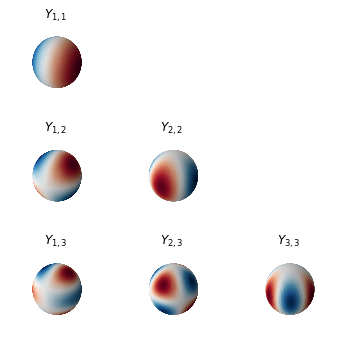
\includegraphics[width=0.5\textwidth]{figures/snap/sph-harm.png} % for .pdf files etc use \includegraphics{test.pdf}
  \caption[Spherical harmonics]{A selection of low order spherical harmonics plotted on a sphere. } %TODO: Add scale!!!
  \label{fig:sphharm}
\end{figure}

Using the spherical harmonics, a sphere surrounding the central atom can be encoded.
To encode density information along the radial direction, spherical harmonics are combined with radial basis functions.
A variety of radial functions can be used for this application.
In \cite{KUHL1982236} the use of a polynomial radial basis is suggested.
However here a set of primitive gaussian type orbitals are used.
This set allows for analytical integration which allows for a significant speedup over numerical integration since it can be precomputed \cite{dscribe}.
These gaussian type orbitals are defined as

$$g_{nl}(r) = \sum_{n'}{n_{max}} \beta_{nn'l} \phi_{n'lr}(r) $$

with 

$$\phi_{nl}(r) = r^l e^{-\alpha_{nl}r^2} $$ %TODO: phi of n oder phi of nl?? / alpha_n oder alpha_nl


\begin{figure} [h]
  \centering
  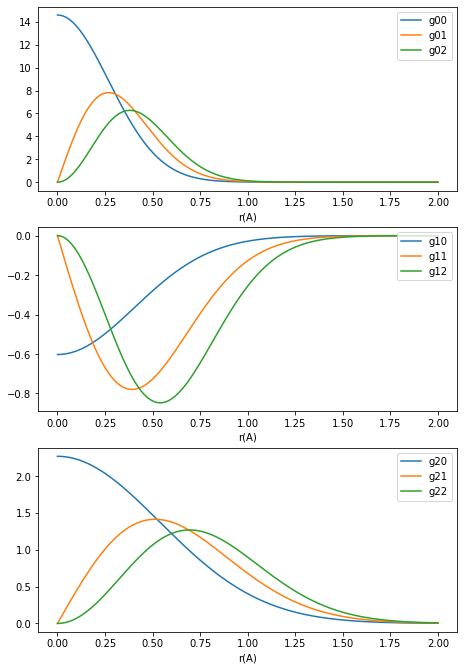
\includegraphics[width=0.5\textwidth]{figures/snap/gaus_orb.png} % for .pdf files etc use \includegraphics{test.pdf}
  \caption[Radial basis functions]{Spherical gaussian orbital functions for a cutoff radius $r_{cut}=2$, $2$, $n_{max}=2$ and $l_{max}=2$. }
  \label{fig:gaussians}
\end{figure}

$\alpha$ and $\beta$ are constants that only need to be computed once for every pair of $l,m, r_{cut}$.
The $\alpha$ parameters control the decay of the radial basis functions at $r_{cut}$.

$\beta_{nn'l}$ parameters orthogonalize the radial basis functions.
For each $l$ the weights $\beta_{nn'l}$ can be computed using the Löwdin orthogonalization:

$$\beta = S(l)^{-1/2} $$

with the entries of the matrix $S$ being defined as

$$S(l)_{nn'} = \langle \phi_{nl} | \phi_{n'l} \rangle  $$

The implementation of $\alpha$ and $\beta$ prefactors is taken from \cite{dscribe} where they are precomputed up to $l \leq 9$.
Higher order factors could be added if needed.


Combining spherical harmonics with radial basis functions the density space surrounding the central atom can be described.
In theory, choosing infinitely high $n, l$ could approximate the space with infinitely high precision.
To get a fixed amount of coefficients, $n_{max}$ and $l_{max}$ need to be chosen that determine the
accuracy of the encoding.
Generally, the higher $n_{max}, l_{max}$ the more accurate the space can be approximated.
%TODO Add figure of the space being described with different n, l , cutoff

For radial basis functions a cutoff radius $r_{cut}$ needs to be defined.
Densities outside this cutoff radius will not be encoded in the features of the space.

The density for every species $Z$ in within the cutoff sphere can be expanded as:

$$ \rho^Z(r) = \sum_{nlm} c^Z_{nlm} g_{nl}(r) Y_{lm}(\theta, \varphi) $$

The coefficients $c_{nlm}^Z$ are features generated by the SNAP descriptor.

$$ c_{nlm}^Z = \iiint_{R^3} g_{nl}(r) Y_{lm}(\theta, \varphi) \rho^Z(r, \theta, \phi)  \,dr\theta\phi   $$
% TODO: Integrate to infinity or r_cut?

The 3 dimensional integral goes over all spherical coordinates within the cutoff sphere.
The coefficients $c^Z_{nlm}$ now describe the 3D space within a fixed size sphere.
\\
The key difference between SNAP and other chemical descriptors is the bi-directional mapping between feature space and 
density space.
From the coefficients, the density space encoded can be easily reconstructed.
This allows for a partial reconstruction of the molecule from the features encoded by SNAP.

However, due to the low number of radial basis functions and spherical harmonics usually used to describe an element, 
the encoding of the density is far from perfect.
While with an infinite amount of coefficients a perfect description of the space is thinkable,
in reality the computational limits only allow for a rather low resolution of the density space [Figure~\ref{fig:snap-density}]. 
\begin{figure} [h]
  \centering
  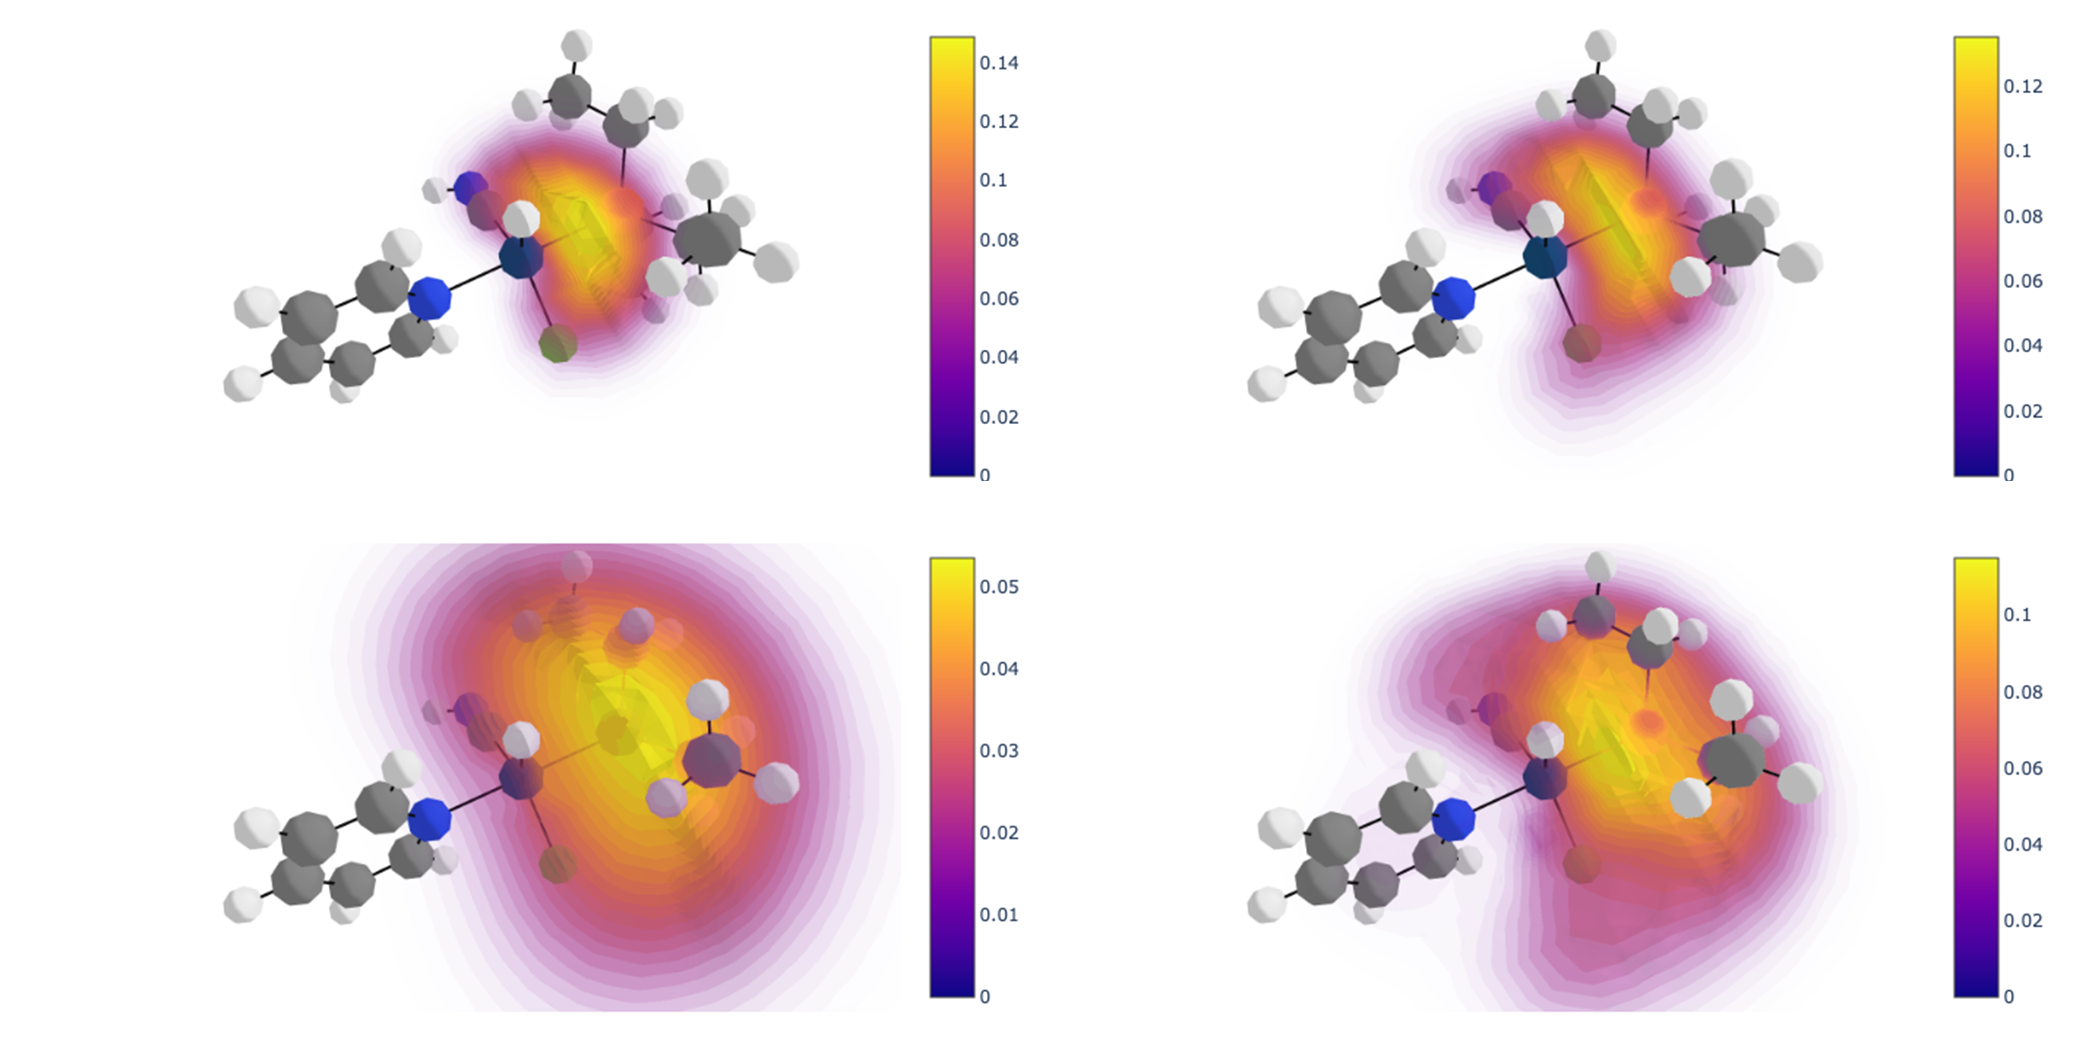
\includegraphics[width=1\textwidth]{figures/snap/density/dense.png} % for .pdf files etc use \includegraphics{test.pdf}
  \caption[SNAP density visualization]{Visualization of the density reconstructed from $c_{nlm}^Z$ coefficients for different resolutions.
  Top: $r_{cut} = 10$, bottom: $r_{cut} = 25$, left: $n_{max} = l_{max} = 2$, right: $n_{max} = l_{max} = 8$.
  The density shown is visualizing the density for phosphorus only.
  The phosphorus atom is the orange atom surrounded by the density cloud.
  }
  \label{fig:snap-density}
\end{figure}

This means that in many cases, the center of the encoded density and the center of the atom do not match.
Especially when the element contains many atoms of one species, the descriptor struggles to fully encode the space.

Despite these issues, predicting the activation barrier from SNAP features is still possible with high accuracy.
The interpretability of these results however is limited to a low resolution.
When using network explainers in combination with SNAP coefficients, this limited accuracy needs to be kept in mind.

%% conclusion.tex
%%

%% ==================
\chapter{Conclusion}
\label{ch:conclusion}
%% ==================

Summary and outlook.


%% --------------------
%% |   Bibliography   |
%% --------------------

\cleardoublepage
\phantomsection
\addcontentsline{toc}{chapter}{\bibname}

\iflanguage{english}
{\bibliographystyle{alpha}}
{\bibliographystyle{babalpha-fl}} % german style

\bibliography{references}


%% ----------------
%% |   Appendix   |
%% ----------------

\cleardoublepage
%% LaTeX2e class for student theses
%% sections/apendix.tex
%% 
%% Karlsruhe Institute of Technology
%% Institute for Program Structures and Data Organization
%% Chair for Software Design and Quality (SDQ)
%%
%% Dr.-Ing. Erik Burger
%% burger@kit.edu
%%
%% Version 1.3.5, 2020-06-26

\iflanguage{english}
{\chapter{Appendix}}    % english style
{\chapter{Anhang}}      % german style
\label{chap:appendix}


%% -------------------
%% | Example content |
%% -------------------
\section{First Appendix Section}
\label{sec:appendix:FirstSection}
		
\setcounter{figure}{0}
		
\begin{figure} [ht]
  \centering
  \caption{A figure}
  \label{fig:anotherfigure}
\end{figure}


\dots
%% ---------------------
%% | / Example content |
%% ---------------------


\end{document}
